\section{Mogan STEM: A WYSIWYG Structured Editor}
\label{sec:mogan}

Mogan STEM is a WYSIWYG structured editor designed to address the limitations of LaTeX while maintaining its strengths in scientific typesetting \cite{moganstem2025, liiistem2025}. The key innovations of Mogan STEM include:

\subsection{Tree-Structured Formulas and Document Structure}
\label{sec:tree-struc-on-mogan}

Unlike LaTeX's linear macro-based representation, Mogan STEM represents documents as structured trees. This enables precise semantic understanding and manipulation of document elements.

\begin{figure}[htbp]
\centering
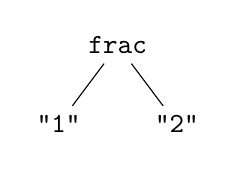
\begin{tikzpicture}[
    level 1/.style={sibling distance=15mm, level distance=10mm},
    every node/.style={align=center}
]
\node {\texttt{frac}}
    child {node {\texttt{"1"}}}
    child {node {\texttt{"2"}}};
\end{tikzpicture}
\caption{The Tree Structure of Mogan Formulas}
\label{fig:frac-tree}
\end{figure}

Figure~\ref{fig:frac-tree} illustrates how mathematical expressions are represented as trees in Mogan STEM. Each node has a specific type and contains its children in a well-defined structure. This representation enables:

\begin{itemize}
    \item Precise cursor positioning and navigation
    \item Structural selection and manipulation
    \item Semantic-aware editing operations
\end{itemize}

\begin{equation}
\label{eq:tree-struc}
\text{Tree}(f) = \begin{cases}
    (\text{leaf}, v) & \text{if } f \text{ is atomic} \\
    (\text{op}, [\text{Tree}(c_1), \ldots, \text{Tree}(c_n)]) & \text{otherwise}
\end{cases}
\end{equation}

Equation~\ref{eq:tree-struc} shows the recursive definition of the tree structure for formulas. Figure~\ref{fig:tree-representation} shows a tree representation of a mathematical expression.

\begin{figure}[htbp]
\centering
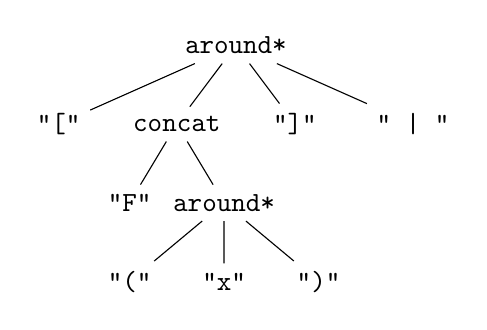
\begin{tikzpicture}[
    level 1/.style={sibling distance=15mm, level distance=10mm},
    level 2/.style={sibling distance=12mm, level distance=10mm},
    level 3/.style={sibling distance=12mm, level distance=10mm},
    every node/.style={align=center}
]
\node {\texttt{around*}}
    child {node {\texttt{"["}}}
    child {node {\texttt{concat}}
        child {node {\texttt{"F"}}}
        child {node {\texttt{around*}}
            child {node {\texttt{"("}}}
            child {node {\texttt{"x"}}}
            child {node {\texttt{")"}}}
        }
    }
    child {node {\texttt{"]"}}}
    child {node {\texttt{" | "}}};
\end{tikzpicture}
\caption{tree representation of $ [F (x)] |$}
\label{fig:tree-representation}
\end{figure}

This tree structure exists at the rendering level, not the syntax level. Figure~\ref{fig:double-line} illustrates image insertion between lines, and Figure~\ref{fig:multiline-mogan} shows Mogan's multi-line data structure.

\begin{figure}[htbp]
\centering
\includegraphics[width=0.3\textwidth]{figure/double-line.png}
\caption{Image insertion between lines}
\label{fig:double-line}
\end{figure}

\begin{figure}[htbp]
\centering
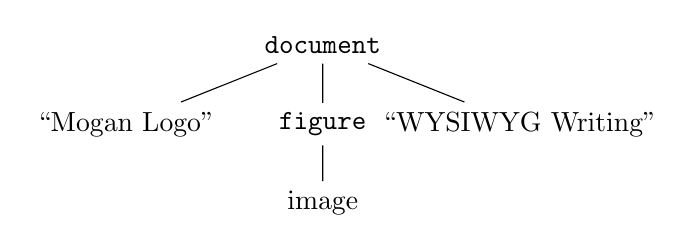
\begin{tikzpicture}[
    level 1/.style={sibling distance=25mm, level distance=10mm},
    level 2/.style={sibling distance=25mm, level distance=10mm},
    every node/.style={align=center}
]
\node {\texttt{document}}
    child {node {``Mogan Logo''}}
    child {node {\texttt{figure}}
        child {node {image}}
    }
    child {node {``WYSIWYG Writing''}};
\end{tikzpicture}
\caption{Mogan's multi-line data structure}
\label{fig:multiline-mogan}
\end{figure}

\subsection{Functional Symbol Representation}

Mogan STEM uses a functional representation for symbols and operators. This provides a clean, compositional semantics for document elements. For example, a fraction is represented as:

\begin{equation}
\label{eq:braket}
\text{frac}(a, b) \mapsto \frac{a}{b}
\end{equation}

This functional approach contrasts with LaTeX's macro-based approach, where \verb|\frac{a}{b}| relies on positional arguments and implicit grouping.

\subsection{Fast Reference Rendering}

Cross-references in Mogan STEM are maintained as bidirectional links in the document tree. When a label is updated, all references to it are automatically updated without requiring a full recompilation. This provides immediate visual feedback and eliminates the need for multi-pass compilation.

\subsection{On-demand plugin loading}

Mogan STEM's architecture supports on-demand loading of features and document types. Unlike LaTeX, where the entire distribution must be installed upfront, Mogan loads only the components needed for the current document. This significantly reduces installation size and startup time.
